\documentclass[11pt]{article}
 
\usepackage[margin=.95in]{geometry} 
\usepackage{amsmath,amsthm,amssymb, graphicx, multicol, array}
 
\newcommand{\N}{\mathbb{N}}
\newcommand{\Z}{\mathbb{Z}}
 

\begin{document}
 
\title{Homework 5}
\author{Juliette Franqueville\\
}
\maketitle

\subsection*{(1) (a)}


\begin{figure}[!h]
    \centering
    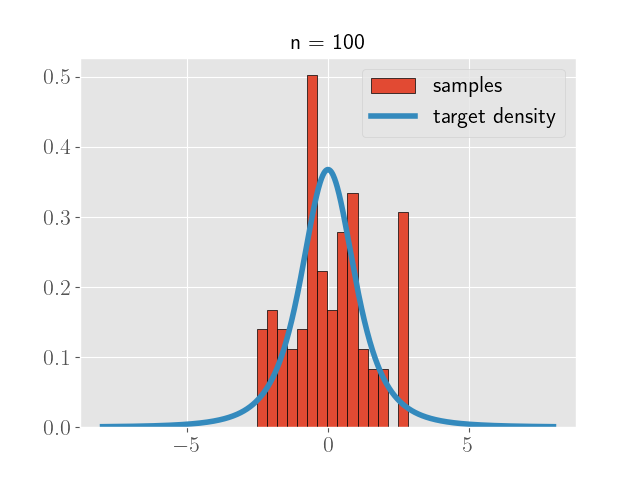
\includegraphics[scale=.5
    ]{../figures/resamples_n_100.png}
    \caption{samples and t distribution for $n=100$}
    \label{fig:my_label}
\end{figure}

\begin{figure}[!h]
    \centering
    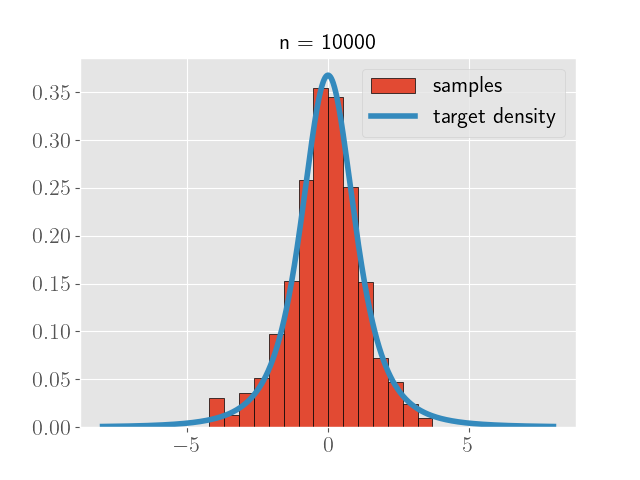
\includegraphics[scale=.5
    ]{../figures/resamples_n_10000.png}
    \caption{samples and t distribution for $n=10,000$}
    \label{fig:my_label}
\end{figure}
\newpage

\subsection*{(b)}
For $n=100$, the estimated mean and variance were 0.12 and 0.84, respectively. For $n=10,000$, they were 0.03 and 1.67. The means were close to the actual mean (0), but the variances were underestimated compared to the actual variance of $t_3$ (3). This is not suprising because the tails of the normal are not as wide as those of the $t$ distribution. In other words, the normal distribution does not fully cover the $t$ distribution, so the points far from the mean in the tails do not get sampled, which makes the variance too small. I redid this exercise with a uniform distribution that  covered $t_3$ better, and the variances were closer to 3.

\subsection*{(2)}
\begin{align*}
    (X_1|X_2) & \propto (X_1, X_2)\\
    & \propto (1-\rho^2)^{-1/2}\text{exp} \left( -\frac{1}{2(1-\rho^2)} \begin{bmatrix} x_1-\mu_1, &x_2-\mu_2 \end{bmatrix} \begin{bmatrix} 1 & -\rho \\ -\rho & 1 \end{bmatrix}\begin{bmatrix} x_1-\mu_1 \\ x_2-\mu_2 \end{bmatrix}\right)\\
    & \propto (1-\rho^2)^{-1/2}\text{exp} \left( -\frac{1}{2(1-\rho^2)}[(x_1-\mu_1)^2-2\rho(x_1-\mu_1)(x_2-\mu_2) + (x_2-\mu_2)^2] \right)\\
     & \propto (1-\rho^2)^{-1/2}\text{exp} \left( -\frac{1}{2(1-\rho^2)}[x_1^2-2x_1(\mu_1+\rho x_2 - \rho x_1)] \right)\\
     & \propto \mathcal{N}(\mu_1 + \rho(x_2-x_1), 1-\rho^2)
\end{align*}

To get $(X_2|X_1)$, we simply swap $X_1$ ad $X_2$. We then use a Gibbs sampler to produce the following plots. I set burn in $=500$ and thin every 2 iterations.

\begin{figure}[!h]
    \centering
    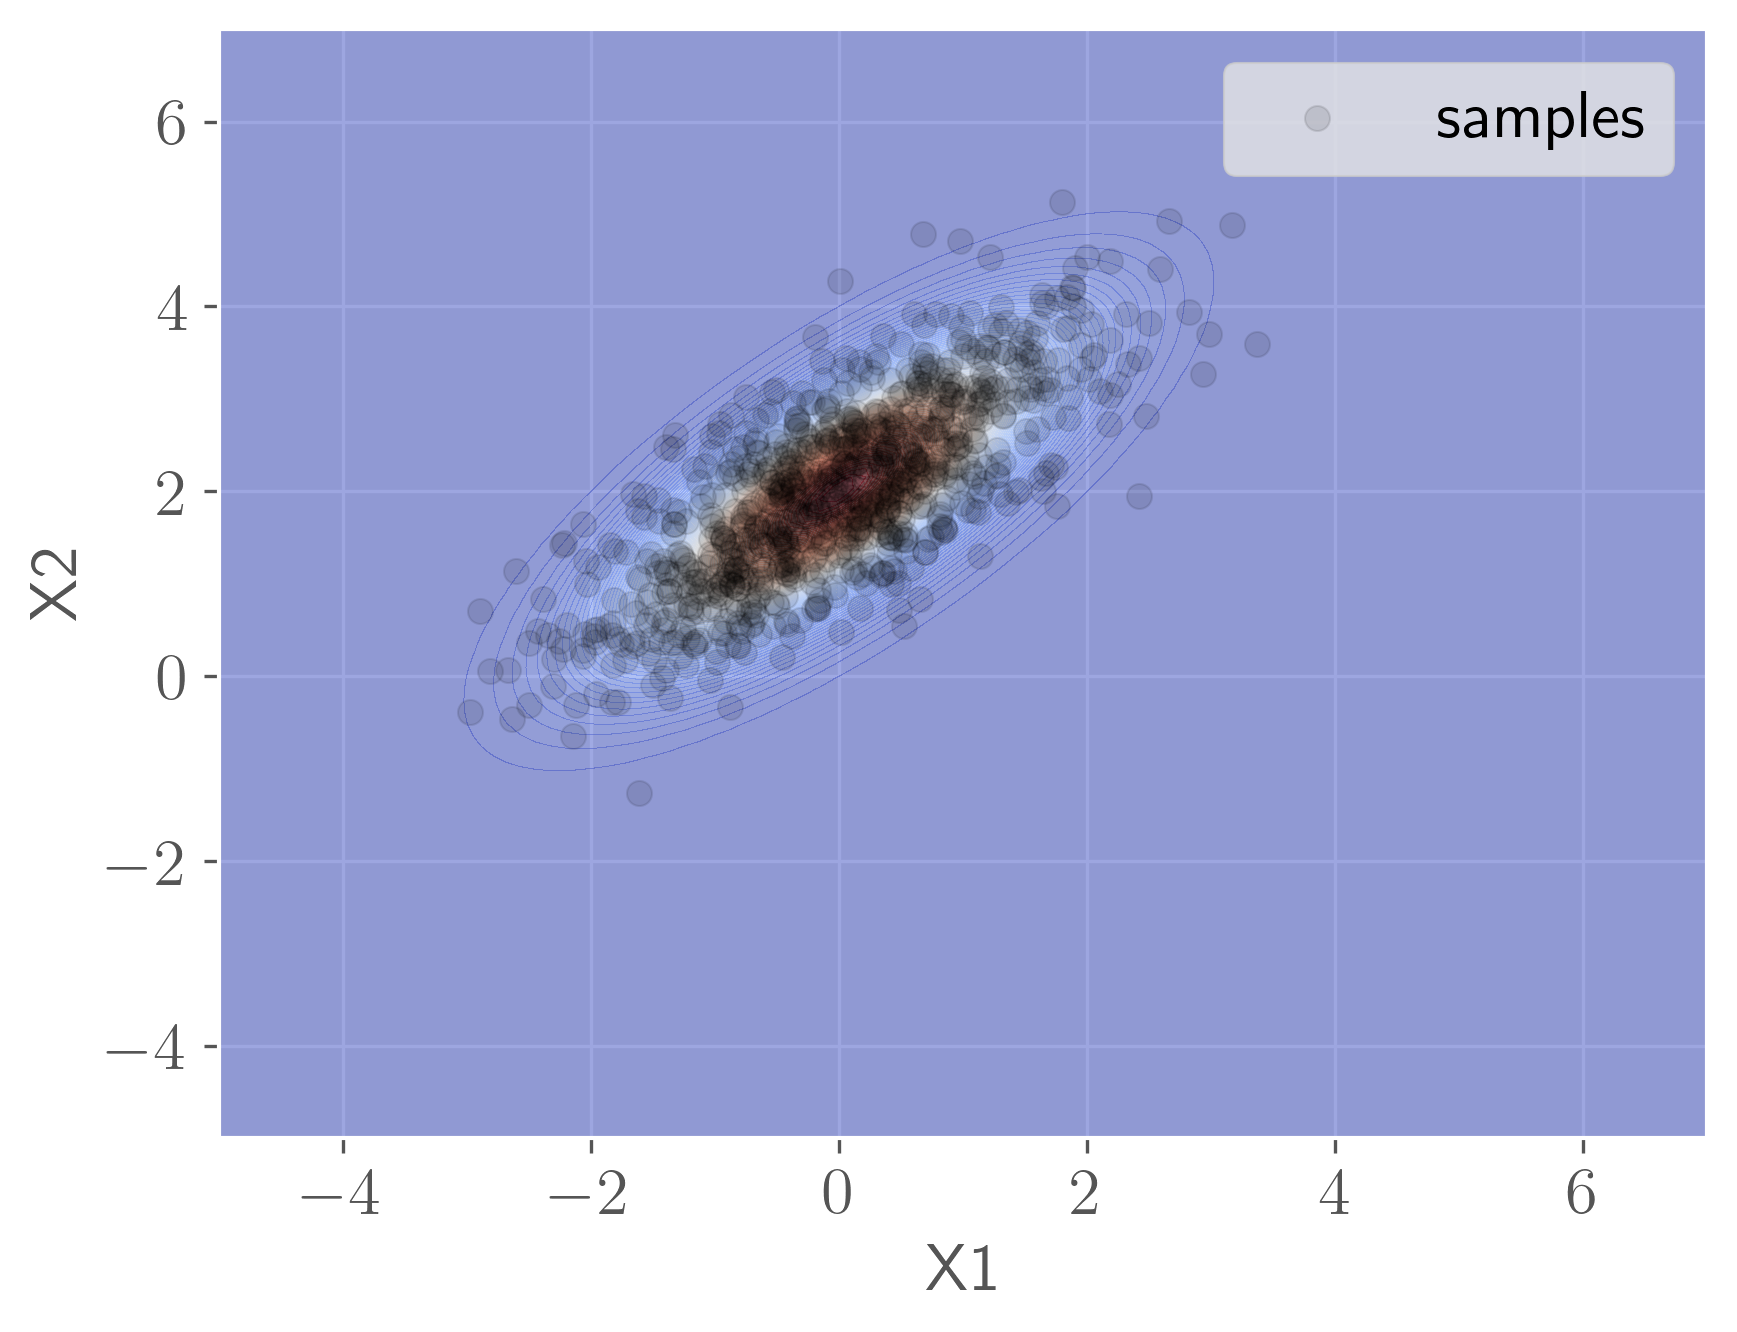
\includegraphics[scale=.6
    ]{../figures/bivar.png}
    \caption{samples and true distribution}
    \label{fig:my_label}
\end{figure}

\begin{figure}[!h]
    \centering
    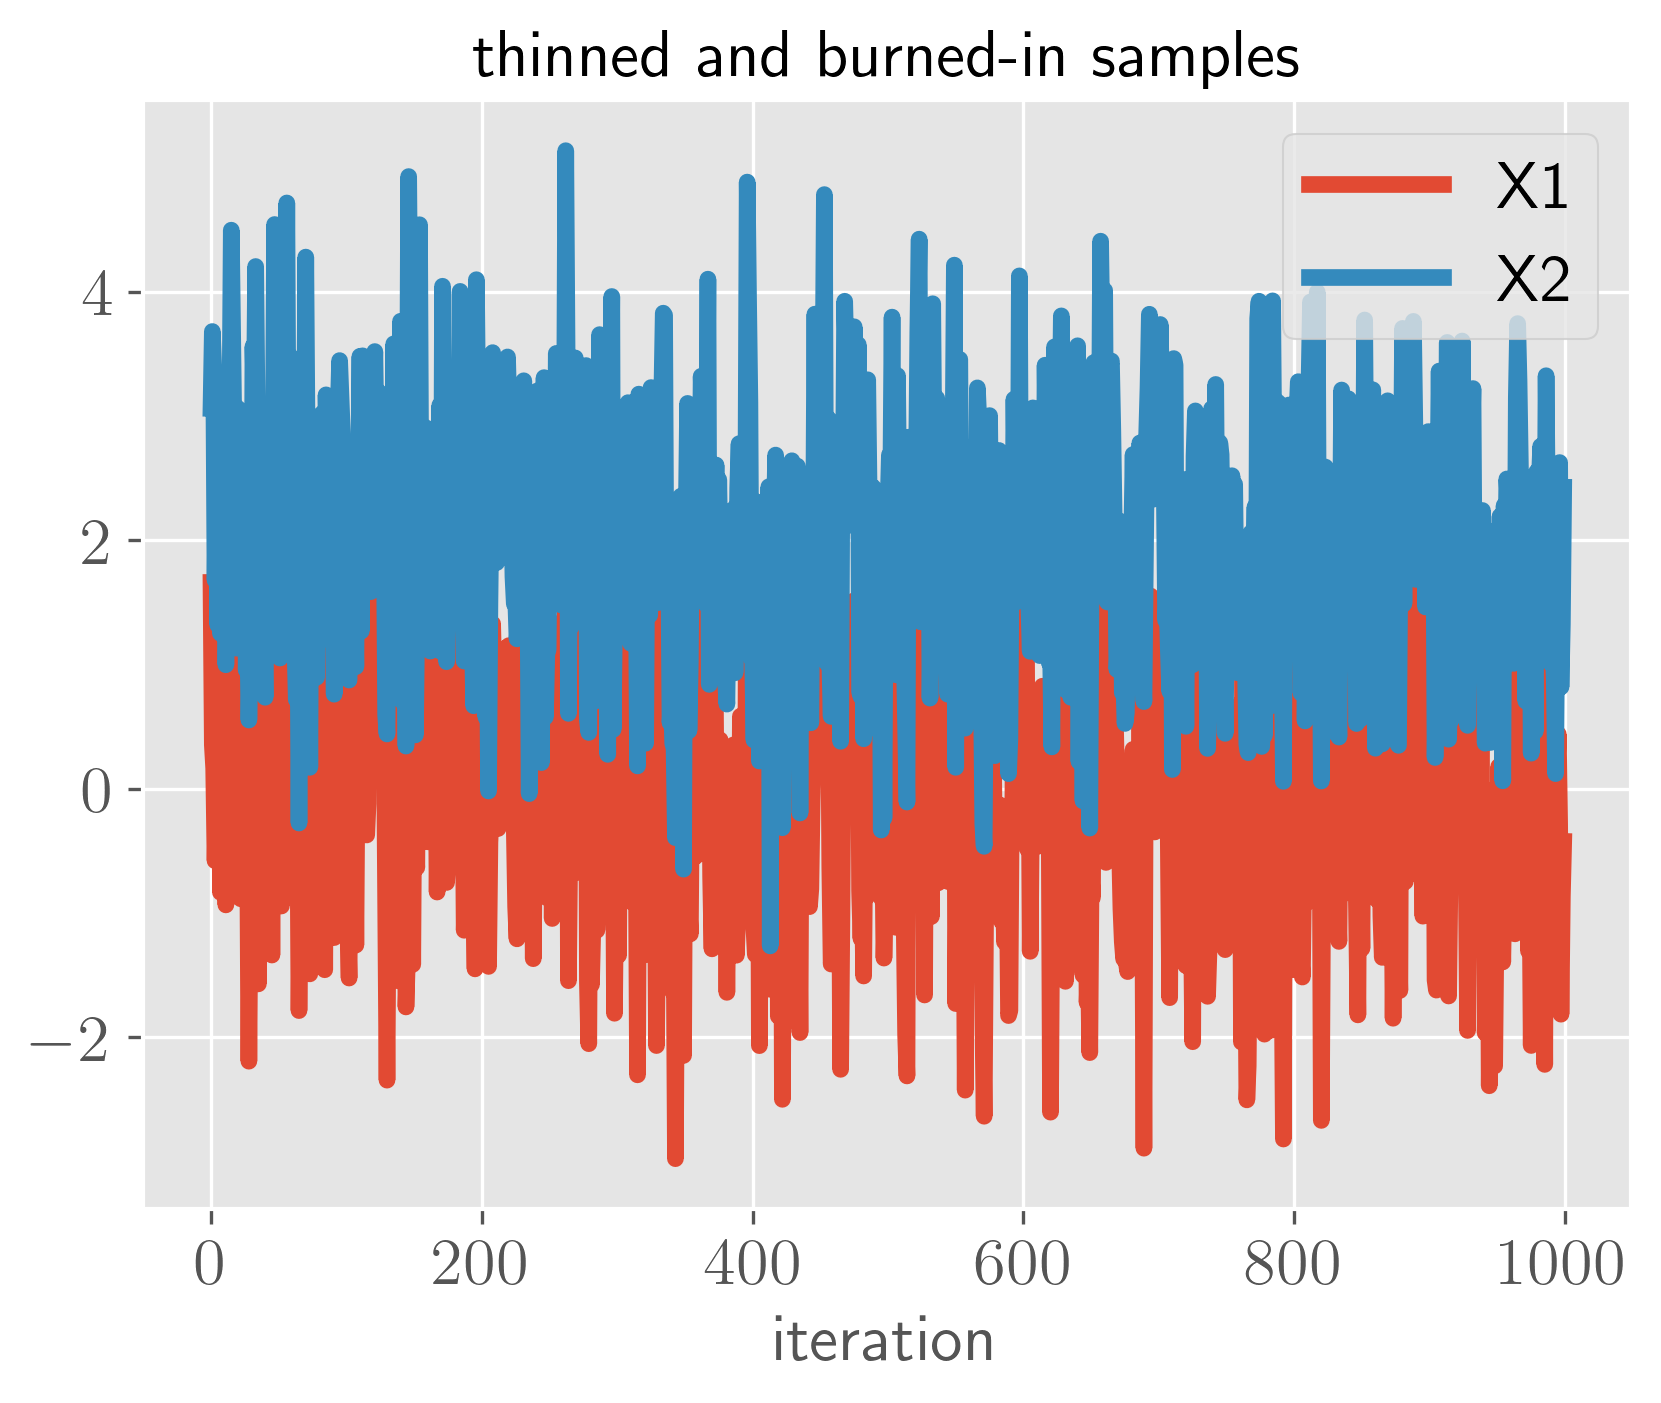
\includegraphics[scale=.6
    ]{../figures/traces.png}
    \caption{Traces}
    \label{fig:my_label}
\end{figure}

\begin{figure}[!h]
    \centering
    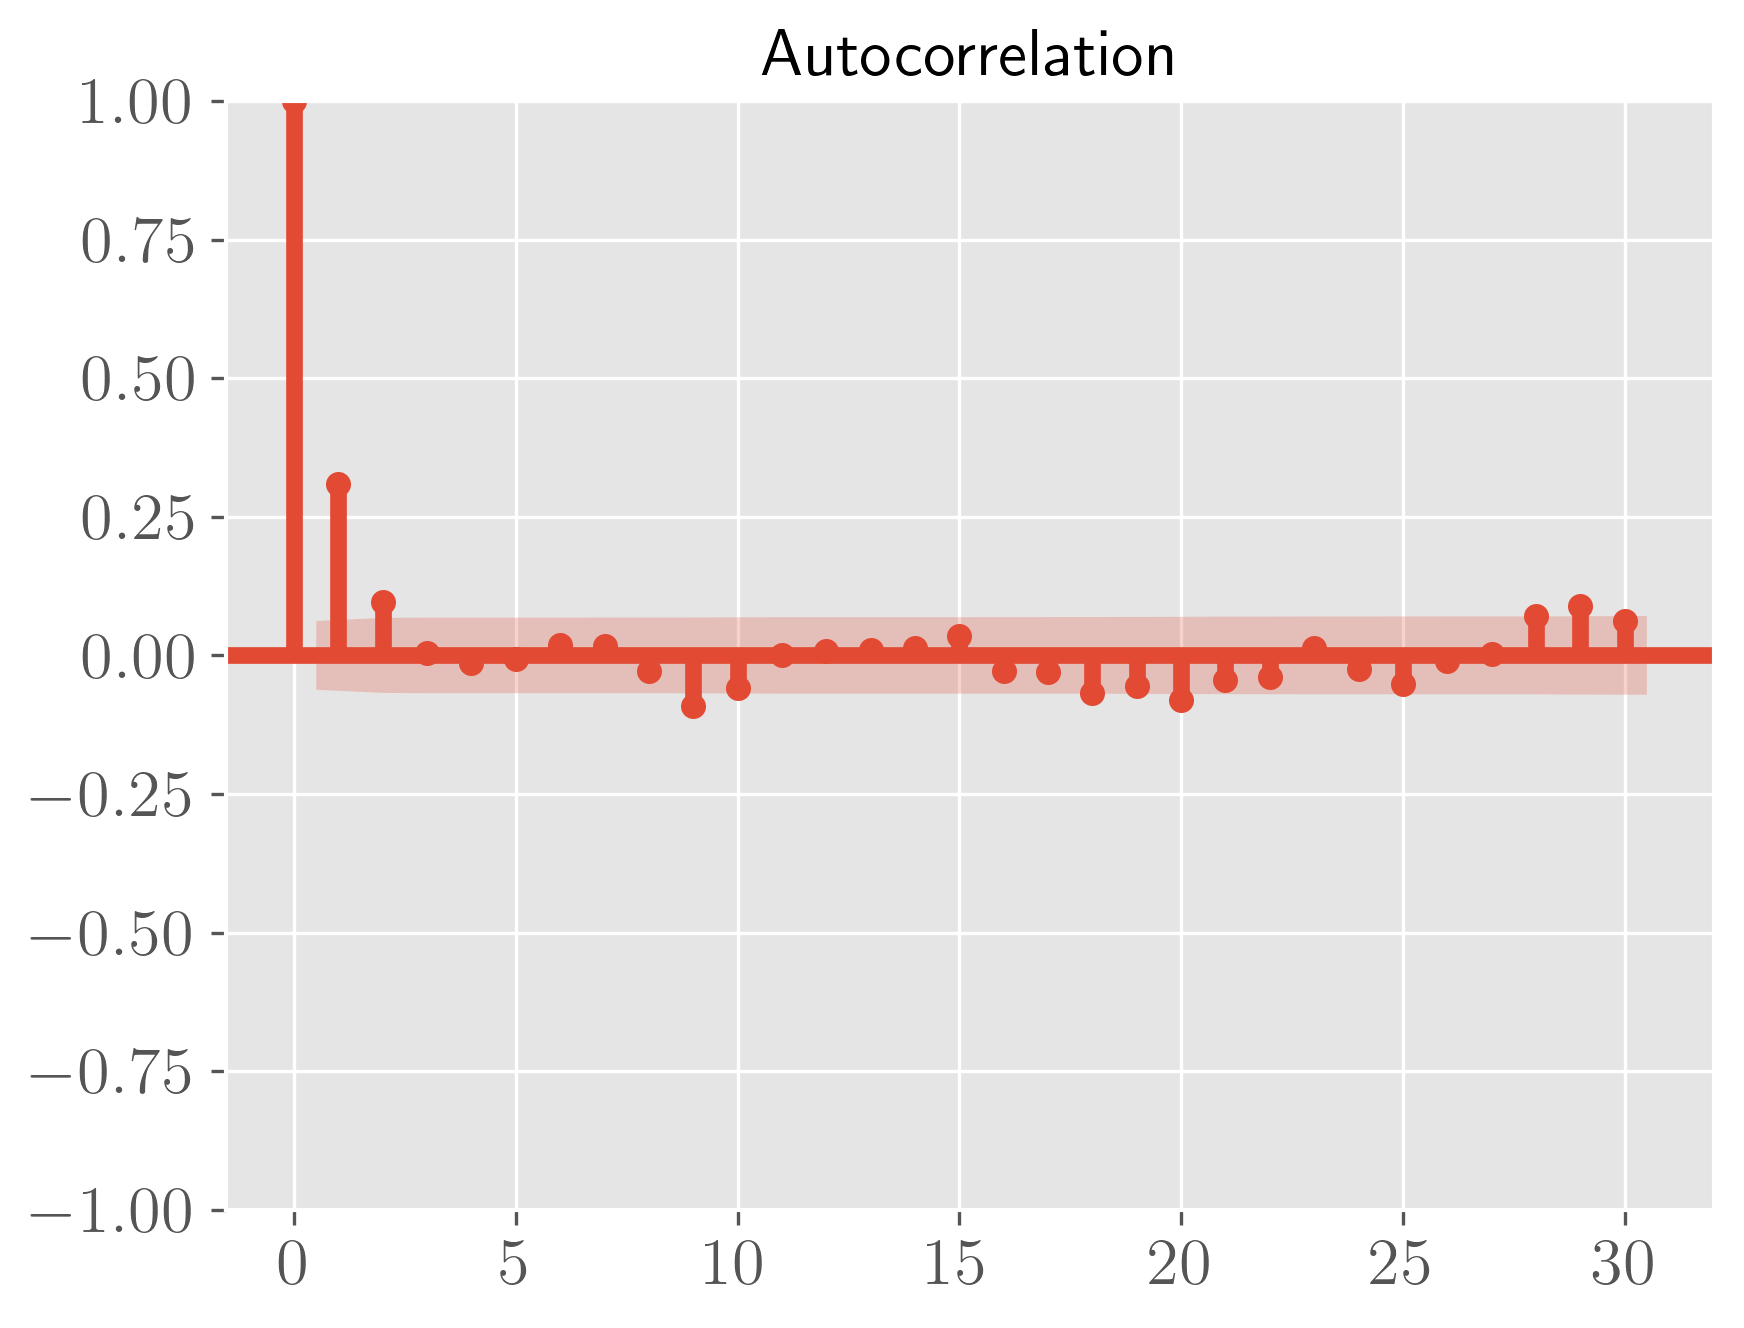
\includegraphics[scale=.6
    ]{../figures/acf1.png}
    \caption{ACF for $X_1$}
    \label{fig:my_label}
\end{figure}

\begin{figure}[!h]
    \centering
    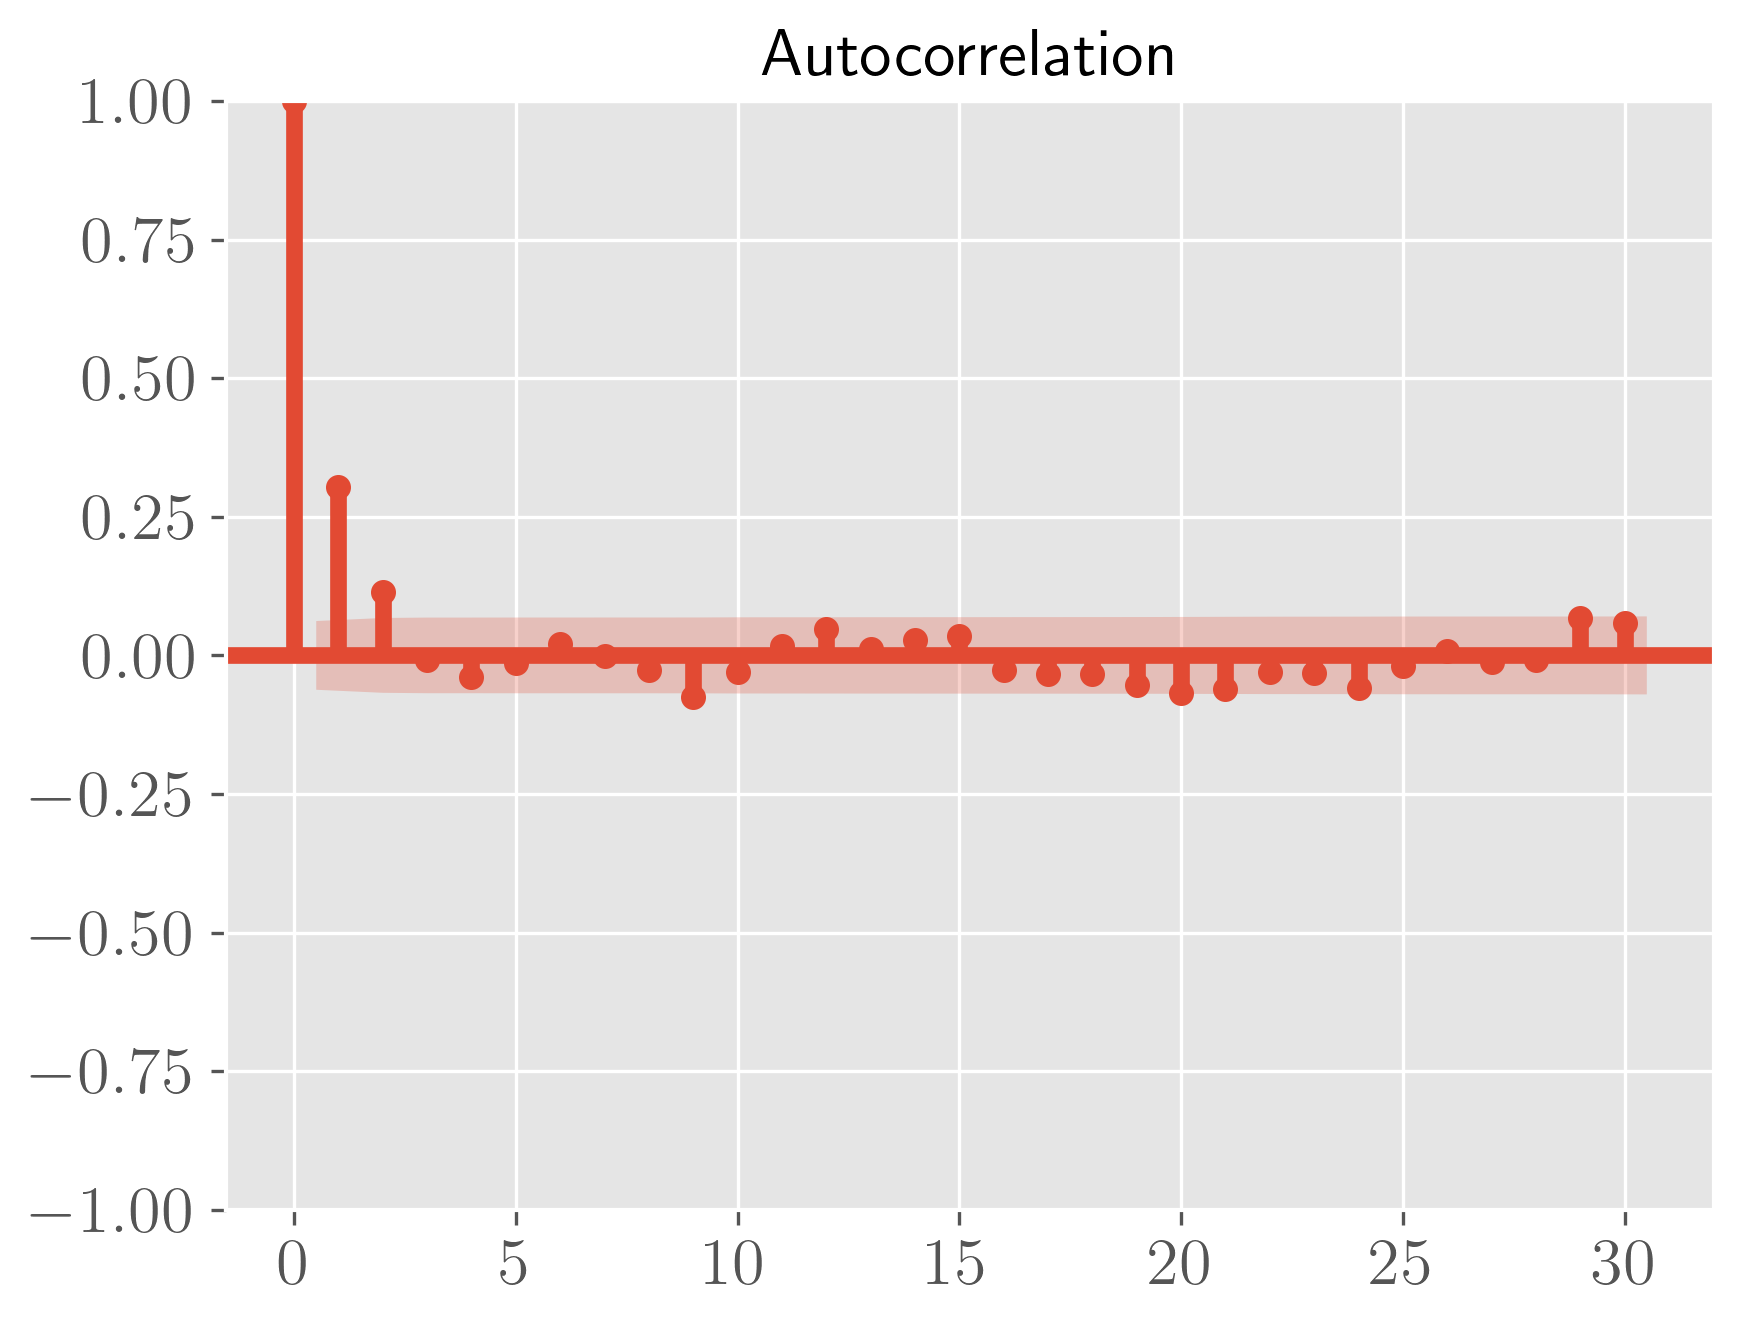
\includegraphics[scale=.6
    ]{../figures/acf2.png}
    \caption{ACF for $X_2$}
    \label{fig:my_label}
\end{figure}
\newpage

\subsection*{(3) (a)}

\begin{align*}
    y_t &= \mu + \rho(y_{t-1} -\mu) + \epsilon_t \\
     var(y_t) &= var(\mu) + var(\rho(y_{t-1} -\mu)) + var(\epsilon_t) \\
     &= \rho^2var(y_{t-1}) + \sigma^2\\
      &= \rho^2var(y_{t}) + \sigma^2\\
      var(y_t) &= \frac{\sigma^2}{1-\rho^2}
\end{align*}

\subsection*{(c)}
\begin{align*}
    E(y_t) &= \mu + \rho E(y_{t-1}) - \mu\rho + E(\epsilon_t)\\
    &= \mu + \rho E(y_{t}) - \mu\rho\\
    E(y_t)[1-\rho] &= \mu[1-\rho]\\
    E(y_t) &= \mu
\end{align*}

\subsection*{(d)}
\begin{align*}
    E(y_t) &= \mu + \rho E(y_{t-1}) - \mu\rho + E(\epsilon_t)\\
    &= \mu + \rho E(y_{t}) - \mu\rho\\
    E(y_t)[1-\rho] &= \mu[1-\rho]\\
    E(y_t) &= \mu
\end{align*}

\subsection*{(4) (a)}
I used 
\begin{align*}
    \rho & \propto \text{constant}\\
    \sigma^2 & \propto IG(\alpha, \beta)
\end{align*}

Note that I could also have used a normal on $\rho$ but this was simpler.

\subsection*{(b)}
Let us rewrite 
\begin{align*}
    y_t \sim \mathcal{N}(\rho y_{t-1}, \sigma^2)
\end{align*}
In vector form as

\begin{align*}
    \boldsymbol{y} \sim \mathcal{N}(\boldsymbol{X}\rho , \sigma^2\boldsymbol{I})
\end{align*}

Then

\begin{align*}
    p(\rho|\boldsymbol{y}, \sigma^2) &\propto p(\boldsymbol{y}|\rho)p(\rho)\\
    & \propto\text{exp} \left( -\frac{1}{2\sigma^2} \sum [y_i-X_i\rho]^2\right)\\
      & \propto\text{exp} \left( -\frac{1}{2\sigma^2} [-2\rho\sumy_iX_i + \rho^2\sum2X_i^2]\right)\\
      & \propto\text{exp} \left( -\frac{\sum X_i^2}{2\sigma^2} [-2\rho\sumy_iX_i/\sum X_i^2 + \rho^2]\right)\\
      & \propto \mathcal{N}(\sum y_i X_i / \sum X_i^2, \sigma^2/\sum X_i^2)
\end{align*}

\begin{align*}
    p(\sigma^2|\boldsymbol{y}, \rho) &\propto p(\boldsymbol{y}|\rho)p(\sigma^2)\\
    &  \propto (\sigma^2)^{-n/2}\text{exp} \left( -\frac{1}{2\sigma^2} \sum [y_i-X_i\rho]^2\right) (\sigma^2)^{-\alpha-1} \text{exp}(-\rho(\sigma^2)^{-1})\\
    &  \propto (\sigma^2)^{-n/2-\alpha-1}\text{exp} \left( -\frac{1}{\sigma^2} [0.5\sum [y_i-X_i\rho]^2 + \beta]\right)\\
    & \propto IG(\alpha + n/2, 0.5\sum [y_i-X_i\rho]^2 + \beta)
\end{align*}

\subsection*{(c)}
I chose $\alpha=\beta=0.5$

\begin{figure}[!h]
    \centering
    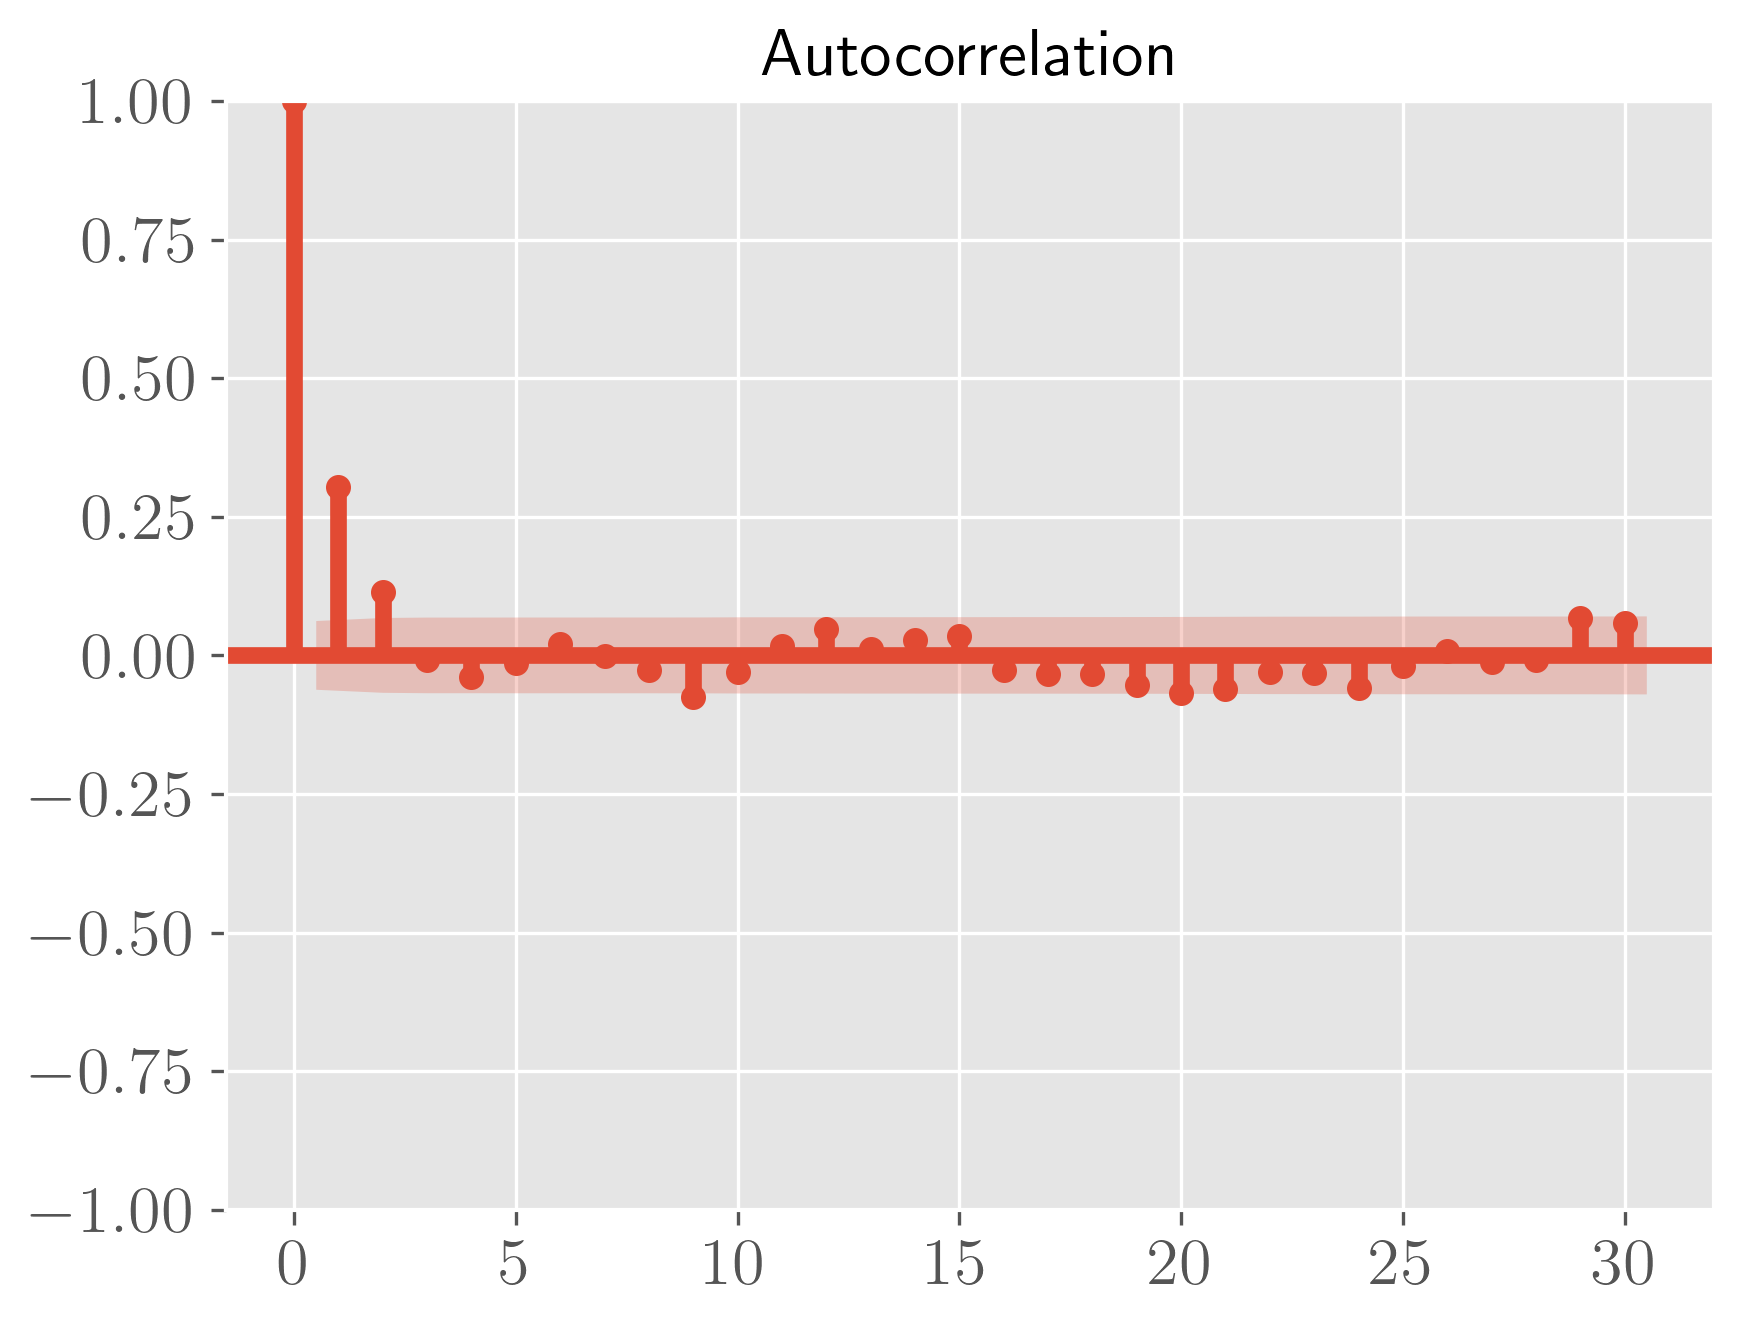
\includegraphics[scale=.6
    ]{../figures/acf2.png}
    \caption{ACF for $X_2$}
    \label{fig:my_label}
\end{figure}

\begin{figure}[!h]
    \centering
    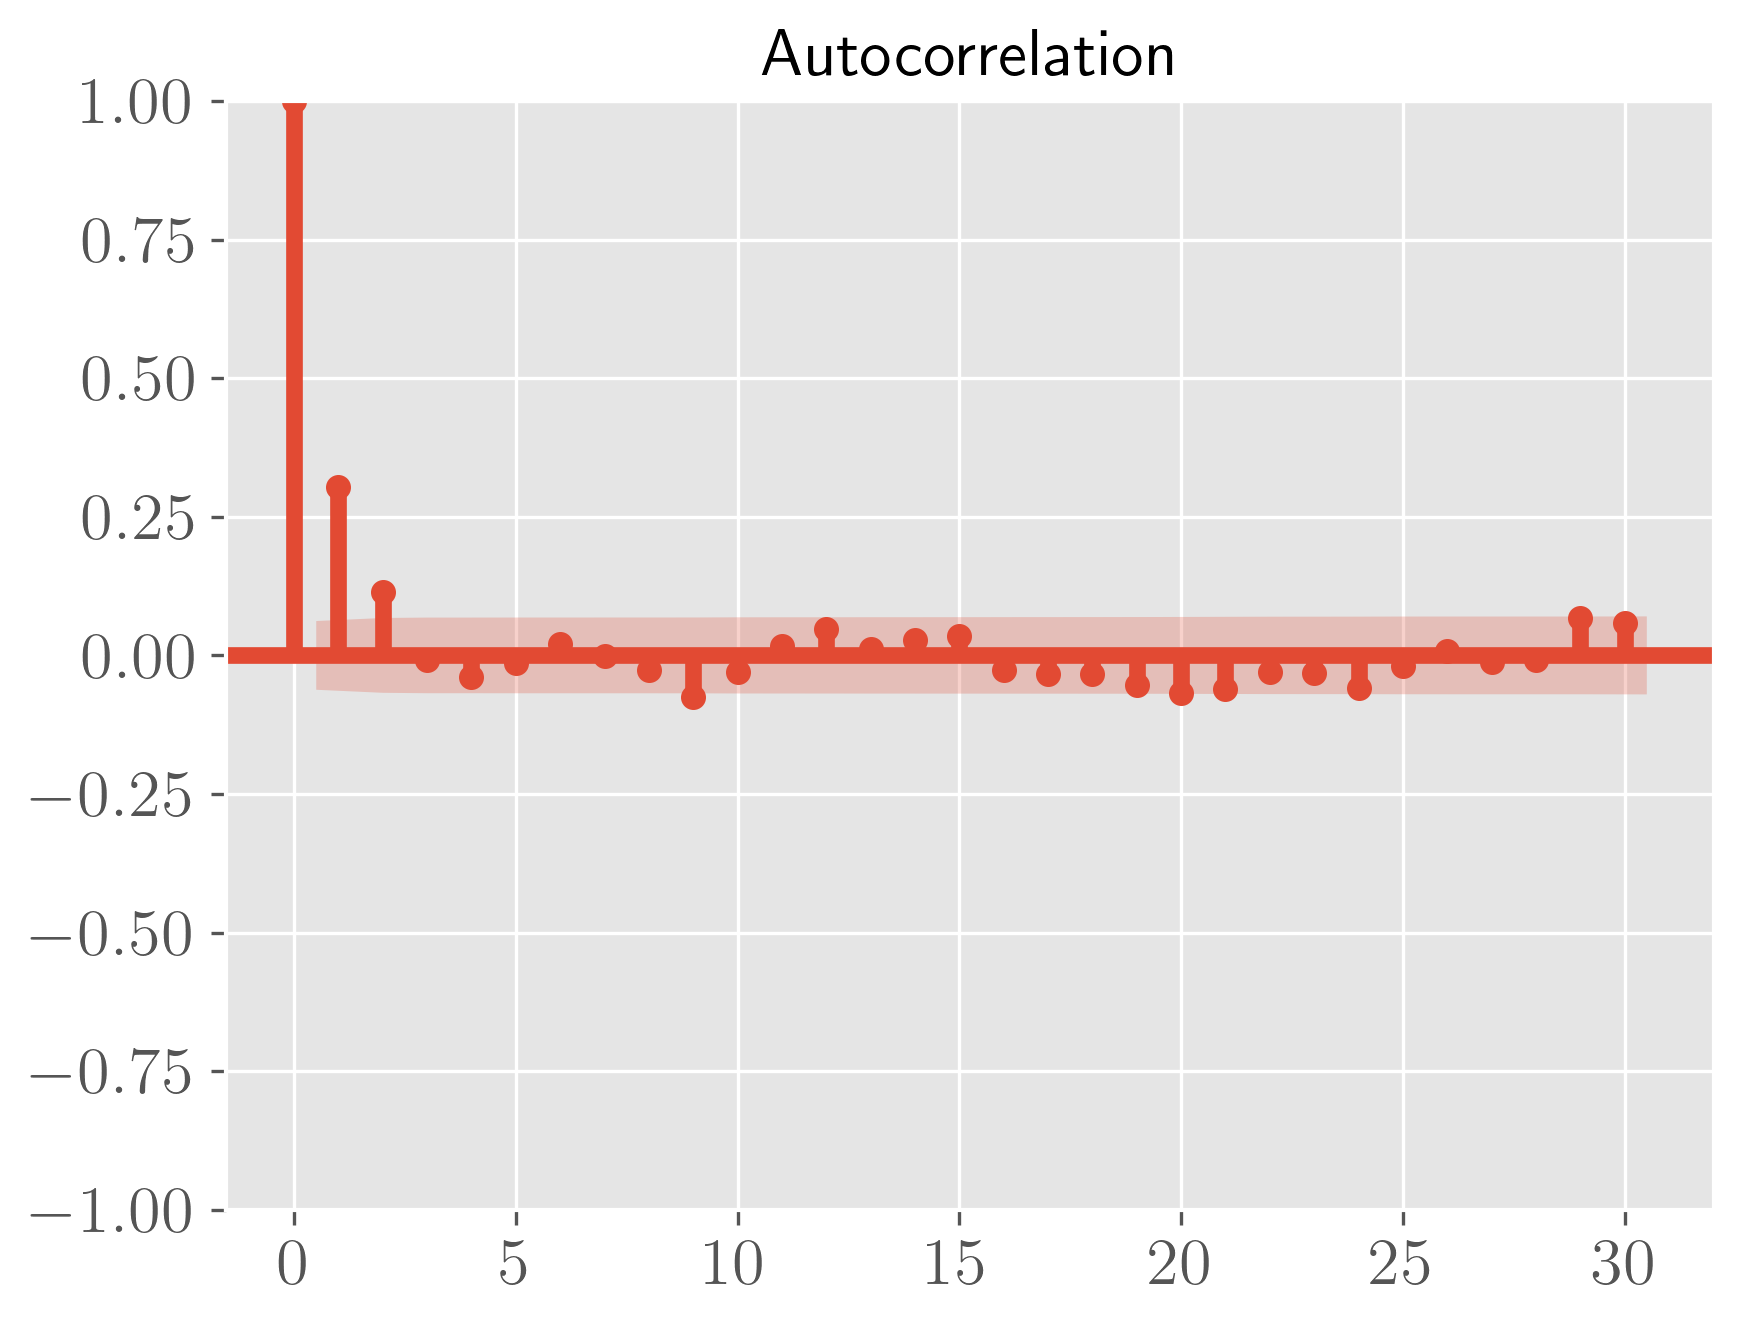
\includegraphics[scale=.6
    ]{../figures/acf2.png}
    \caption{ACF for $X_2$}
    \label{fig:my_label}
\end{figure}

\end{document}
